\chapter{Coleta de Dados}
\label{cap:metodologia}

O objetivo deste trabalho é analisar as \textit{breaking changes} no ecossistema do \gls{npm}. Para realizar isso, de um conjunto de dados sobre os pacotes do \gls{npm}, descrito na Seção \ref{sec:col_base}, foi utilizada uma amostra aleatória representativa, conforme explicado na Seção \ref{sec:col_amostra}. Dessa amostra, cada um dos pacotes foram copiados localmente -- coincidentemente, todos os pacotes estavam hospedados no \textit{GitHub} -- e todas as \textit{releases} que continham alterações de provedores foram executadas, através dos comandos \textit{npm install/npm test}, para detectar se continham algum erro, conforme a Seção \ref{sec:bcdetect} explica. Após executarem, os pacotes e \textit{releases} que resultaram em algum erro foram separados em \textit{erros internos} e \textit{breaking changes}, conforme a Seção \ref{sec:col_dados}.

\section{Coleta do Conjunto de Dados}
\label{sec:col_base}
O conjunto de dados utilizado neste trabalho foi extraído do registro do \gls{npm}\footnote{https://registry.npmjs.org/}. Desse registro, foram recuperados os arquivos metadados \textit{package.json} de 461,548 pacotes publicados no período de 20 de Dezembro de 2010 até 01 de Julho de 2017. Os principais dados recuperados no \textit{package.json} são os \textit{timestamp} de cada uma das \textit{releases} dos pacotes, os provedores que o cliente continha em cada \textit{release} e suas respectivas versões. A Figura \ref{fig:package_json} exibe as informações do pacote \textit{buffer-includes}\footnote{http://registry.npmjs.org/buffer-includes} que podem ser recuperadas de seu \textit{package.json}.

\begin{figure}
    \centering
    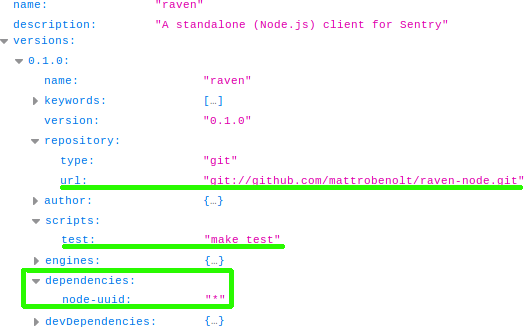
\includegraphics[scale=0.5]{figuras/package_json.png}
    \caption{Informações que serão recuperadas do \textit{package.json} para validar um pacote}
    \label{fig:package_json}
\end{figure}{}

A partir do \textit{timestamp} de uma \textit{release} qualquer, foram resolvidas as versões de cada um dos provedores que o cliente aceitava no momento de sua \textit{release}. Através dessa \textit{timestamp}, foi possível identificar qual a última versão de cada provedor que o cliente aceitava quando publicou sua \textit{release}. Por fim, foram excluídos desta base de dados todos os pacotes que não continham nenhum provedor, pois quando um pacote não contém provedores, não há como sofrer com \textit{breaking changes}. Dessa maneira, a base final contém um total de 366,629 pacotes do \gls{npm}.

\section{Coleta da Amostra}
\label{sec:col_amostra}
% para remover a lista de siglas, foi utilizado um \textit no http
Para este trabalho, foi utilizada uma amostra do conjunto de dados que foi especificado na Seção \ref{sec:col_base}, que contém um total de \textit{366K} pacotes e por isso, realizar uma análise manual para essa quantidade de pacotes não é viável. Por isso, será utilizada uma amostra representativa contendo 384 pacotes, com base em um cálculo amostral\footnote{https://pt.surveymonkey.com/mp/sample-size-calculator/} com 95\% de confiança e $\pm$5\% de margem de erro. De cada pacote sorteado aleatoriamente, foi recuperado o seu arquivo metadado \textit{package.json} e verificado se o pacote cumpre três requisitos: possuir um \textit{script} de teste não vazio e diferente do \textit{script} padrão de teste do \gls{npm}: \textit{Error: no test specified}; possuir a \textit{url} do repositório do pacote; e o repositório do pacote precisa existir -- será esperado de uma requisição \textit{HyperText Transferer Protocol} (HTTP) para o repositório o código \textit{200} indicando sua existência. Todos esses requisitos foram analisados recuperando a última \textit{release} disponível.

Em 33 dos 384 pacotes não foi possível executar o comando \textit{npm install}/\textit{npm test} para nenhuma de suas \textit{releases}. Desses 33 pacotes, 15 não possuíam algum dos arquivos necessários para os testes; 10 continham \textit{scripts} de teste inválidos em todas as suas \textit{releases}, tal como \textit{test: "no tests"}\footnote{https://github.com/djoulz22/drbd/blob/4920434f92656e6a49f09a56ef7eb4978ba6253c/package.json\#L7}; 4 haviam listados alguns dos arquivos no \textit{.gitignore} -- arquivo utilizado pelo \textit{git} para ignorar arquivos no repositório --, mas que eram necessários para a execução; 2 necessitaram de configurações específicas em banco de dados e não foi possível realizá-las; 1 pacote foi considerado como um \textit{toy package}, ou seja, não era um projeto real, apenas um repositório com um único arquivo; e 1 pacote requeria uma variável de ambiente para acessar um determinado site. Dessa forma, os 33 pacotes foram substituídos em um novo sorteio seguindo o mesmo critério, totalizando 384 pacotes com 4544 \textit{releases} que foram utilizados no estudo. Um detalhe importante se refere aos pacotes que utilizavam algum tipo de sistemas de banco de dados como o \textit{MySql\footnote{https://www.mysql.com}}. Quando um erro foi ocasionado pela falta de um destes sistemas, então esses sistemas foram iniciados e o pacote foi re-executado. Somente quando o pacote necessitava de uma configuração específica e que não foi possível configurá-la, o pacote foi substituído por outro.

\section{Detecção de \textit{Breaking Changes}}
\label{sec:bcdetect}
Para este trabalho, foi desenvolvida uma ferramenta chamada \textit{BCDetect} disponível no \textit{GitHub}\footnote{https://github.com/danielventurini/bcdetect} sob a licença \textit{MIT}\footnote{https://choosealicense.com/licenses/mit}. Esta ferramenta clona o repositório do respectivo pacote e cria uma estrutura de dados para armazenar as informações sobre o pacote, na qual cada \textit{release} contém seus \textit{timestamps} e todas os provedores com suas versões resolvidas e tipo de atualização que os provedores realizaram desde a última \textit{release} do cliente -- \textit{steady} significa que o provedor não publicou nenhuma \textit{release} aceita pelo cliente; \textit{upgrade} significa que o provedor publicou uma nova \textit{release} desde a última \textit{release} do cliente; e quando não há nenhuma dessas informações, o provedor foi inserido no \textit{package.json} nesta \textit{release}. Essa estrutura está representada na Figura \ref{fig:bc_work}, que seria construída a partir dos dados do pacote \textit{buffer-includes} da Figura \ref{fig:package_json}.

\begin{figure}
    \centering
    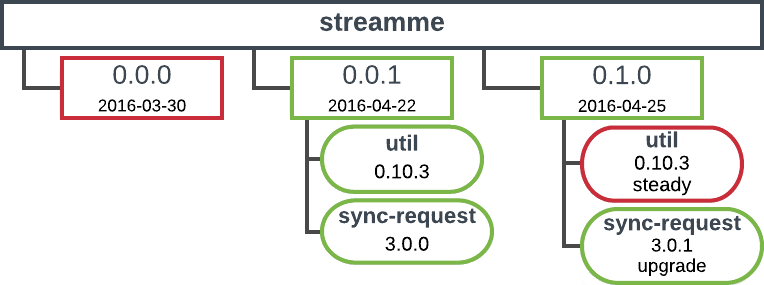
\includegraphics[scale=2]{figuras/bcdetect_work.png}
    \caption{Estrutura de dados para representar o pacote \textit{buffer-includes}}
    \label{fig:bc_work}
\end{figure}{}

Se uma \textit{release} só contém provedores que não foram atualizados (\textit{steady}) desde a \textit{release} anterior do cliente, então essa \textit{release} não é executada. Se uma \textit{release} do cliente houver provedores adicionados ou com novas versões aceitas (\textit{upgrade}), então essa \textit{release} é executada. Após clonado o repositório, é executado o comando \textit{git checkout} com o \textit{timestamp} da \textit{release} do cliente, fazendo com que todos os arquivos sejam restaurados para exatamente os mesmos arquivos do momento em que o cliente publicou a \textit{release}. Então o arquivo \textit{package-lock.json}\footnote{https://docs.npmjs.com/files/package-lock.json} é excluído, pois esse arquivo altera o comportamento do comando \textit{npm install} -- a partir do \textit{NPM@5} -- fazendo com que o \gls{npm} instale as versões dos provedores de acordo com o \textit{package-lock.json}, e não de acordo com o \textit{package.json}. Após, os provedores e suas respectivas versões são adicionados no campo \textit{dependencies} do \textit{package.json} e os demais campos são removidos\footnote{campos para dependências no \textit{package.json}, tais como o \textit{peerDependencies}, \textit{optionalDependencies} e o \textit{globalDependencies}}. Esta operação não diferencia os provedores que estão no \textit{dependencies} ou no \textit{devDependencies}, uma vez que, para realizar o \textit{test}, ambos os provedores são requeridos. Por fim, é alterado a versão do \textit{Node.js} para a versão contida no campo \textit{engines\textrightarrow node} -- se houver -- do \textit{package.json} ou para a versão mais recente utilizando como referência o \textit{timestamp} da \textit{release} do cliente. Por fim, os comandos \textit{npm install/npm test} são executados.

O chaveamento de versões do \textit{Node.js} é necessário pois as versões \textit{releases major} do \textit{Node.js} não são retro-compatíveis, ou seja, um pacote que executa com sucesso na versão \textit{0.x} do \textit{Node.js}, por exemplo, provavelmente não irá executar com sucesso na versão \textit{8.x} do \textit{Node.js}. Desta forma, toda vez que os comandos \textit{npm install/npm test} resultam em erro, é alterado a versão do \textit{Node.js} para a próxima \textit{release major} inferior e novamente é executado os comandos. Analogamente, esse problema de versões atinge o \gls{npm}, mas ao alterar a versão do \textit{Node.js}, a versão do \gls{npm} é atualizado também. Para realizar a alteração da versão do \textit{Node.js} é utilizado como referência o \textit{timestamp} da \textit{release} do cliente. Através desse \textit{timestamp}, é possível identificar a última \textit{release} do \textit{Node.js} disponível\footnote{https://nodejs.org/en/download/releases} no momento da \textit{release} do cliente, ou seja, qual é a \textit{release} máxima do \textit{Node.js} que o cliente executou o pacote. Assim, o pacote é executado em todas as versões \textit{major} do \textit{Node.js}, da versão mais atual, pelo \textit{timestamp} da \textit{release} do cliente, até a versão \textit{major} mais antiga. Para o pacote da Figura \ref{fig:bc_work}, a sua \textit{release 0.1.0} possui o \textit{timestamp 2015-10-28}, e a última \textit{release} do \textit{Node.js} disponível até esta data é a \textit{4.2.1}. Assim, esse pacote foi executado com as \textit{releases 4.x, 3.x, 2.x, 1.x, 0.x} do \textit{Node.js}, até que uma dessas resultassem em sucesso na execução. Por fim, o \textit{BCDetect} salva as seguintes informações:

\begin{itemize}
    \item versão do cliente;
    \item se houve alteração na versão aceita de alguns dos provedores;
    \item os códigos da execução do \textit{npm install} e \textit{npm test} -- sucesso ou erro;
    \item a versão do \textit{Node.js} que deveria ser executado com base na data da \textit{release}; e
    \item a versão do \textit{Node.js} que realmente o pacote executou com sucesso.
\end{itemize}{}

\section{Dados da Execução dos Pacotes}
\label{sec:col_dados}
% o parser do filipe tinha um erro que não resolvia dependências com versões alpha, beta, rc, ..., por exemplo x.y.z-aplha.1 não era resolvido, somente versões x.y.z. Então, houve alguns erros justamente por não haverem as dependências. Quando o erro foi por causa disso, eu desconsiderei que houve erro, ou seja, eu simplesmente resolvi a dependência, refiz o install/test.

% tabela considerando os erros por pacotes não resolvidos:
% não é uma tabela válida, mas apenas para manter o controle.
% \begin{table}[]
% \centering
% \begin{tabular}{|l|l|l|}
% \hline
%                     & Pacotes & \textit{Releases} \\ \hline
%     Total           & 384     & 4544     \\
%     Executado       & 384     & 2374     \\
%     Não executado   & 0       & 2242     \\
%     Sucesso         & 142     & 901     \\
%     Erro            & 242     & 1473     \\ \hline
% \end{tabular}
% \caption{Resultado da execução, por pacotes e \textit{releases}}
% \label{tab:res_rq1}
% \end{table}

% 20 pacotes sofreram com esse problema, resultando em 101 erros que ocorreram por causa do parser. Além, mais 58 release resultaram em erro apenas porque o parser não recuperou alguma dependência. Assim, os dados abaixo estão considerando que esses erros não ocorreram

Ao todo, 384 pacotes clientes foram utilizados nesta pesquisa e foram executadas o \textit{script install/test} em pelo menos uma de suas \textit{releases}. Desses 384 pacotes, 220 resultaram em erros para alguma de suas \textit{releases}. Já analisando os resultados por \textit{releases}, de todas as 4544, foram executadas um total de 2332 \textit{releases}, enquanto que 2242 \textit{releases} não foram executadas pois não haviam alterações nas \textit{releases} dos provedores, ou não continham algum \textit{script} de teste válido. Após o término da execução, 1018 \textit{releases} executaram com sucesso, enquanto que 1314 \textit{releases} resultaram em erros no \textit{script install/test}. A Tabela \ref{tab:res_rq1_1} contém os resultados prévios sem que os pacotes que resultaram em erro fossem analisados, ou seja, são dados apenas da execução dos pacotes.

\begin{table}[]
\centering
\begin{tabular}{|l|l|l|}
\hline
                    & Pacotes & \textit{Releases} \\ \hline
    Total           & 384     & 4544     \\
    Executado       & 384     & 2332     \\
    Não executado   & 0       & 2242     \\
    Sucesso         & 164     & 1018     \\
    Erro            & 220     & 1314     \\ \hline
\end{tabular}
\caption{Resultado da execução, por pacotes e \textit{releases}}
\label{tab:res_rq1_1}
\end{table}

Após executarem, todas as 1314 \textit{releases} que resultaram em erros foram analisadas manualmente para separar os erros falso-positivos dos erros reais. Conforme explicado na Seção \ref{sec:qp1:approach}, os erros do tipo falso-positivos são erros que foram gerados pela falta de alguma configuração, isso é, devido uma má configuração, o execução da \textit{release} resultou em erros. Os erros falso-positivos mais comuns estavam relacionados a serviços que necessitavam de configurações prévias, tais como o \textit{mysql} e o \textit{mongodb}, que por vezes necessitavam de tabelas, senhas, \textit{scripts}, entre outras configurações para que os pacotes executassem com sucesso. Após as \textit{releases} serem analisadas manualmente, foi constatado um total de 37 pacotes com falso-positivos em todas as suas \textit{releases}, totalizando 172 \textit{releases} e mais 238 \textit{releases} que impactaram parcialmente outros pacotes, ou seja, não foram o único tipo de erro no pacote. Assim, todos os 37 pacotes e as 410 \textit{releases} foram consideradas como se estivessem executadas com sucesso. Dessa maneira, após a análise prévia, os dados atualizados são mostrados na Tabela \ref{tab:res_rq1_2}.

\begin{table}[]
\centering
\begin{tabular}{|l|l|l|}
\hline
                    & Pacotes & \textit{Releases} \\ \hline
    Sucesso         & 201     & 1428     \\
    Erro            & 183     & 904     \\ \hline
\end{tabular}
\caption{Resultado da execução, contabilizando os falso-positivos, por pacotes e \textit{releases}}
\label{tab:res_rq1_2}
\end{table}

Então, foi realizada a última etapa da análise dos pacotes para se confirmar a origem do erro: uma chamada à uma função do provedor que contém uma \textit{breaking change} ou alguma alteração realizada pelo cliente. Do total de 183 pacotes com erro, 96 sofreram casos de erros internos, enquanto que 45 pacotes sofreram algum dos casos particulares de \textit{breaking change}. Por fim, 39 pacotes sofreram \textit{breaking changes} em uma de suas \textit{releases}. Também, em 31 pacotes houveram alguma \textit{release} da qual não foi encontrado o motivo do erro. Porém, um pacote que sofreu uma \textit{breaking change}, por exemplo, pode ter sofrido também com erros internos, e vice-versa, pois um caso não influência na ocorrência dos demais. Por isso, os resultados são melhores apresentados em função das \textit{releases}, uma vez que as \textit{releases} só podem sofrer com apenas um tipo de erro. Dessa maneira, do total de 904 \textit{releases} que sofreram algum erro, foram identificadas 428 \textit{releases} com erros internos, 213 \textit{releases} com erros dos casos particulares de \textit{breaking changes}, 190 erros do caso de \textit{breaking changes} e em 73 \textit{releases} não foi possível descobrir o motivo que gerou o erro. A Figura \ref{fig:res_rq1_g} contém todos os dados dos resultados. Assim, os dados sobre os pacotes e \textit{releases} que sofreram com \textit{breaking changes} serão utilizados para responder as questões de pesquisa.

\begin{figure}
    \centering
    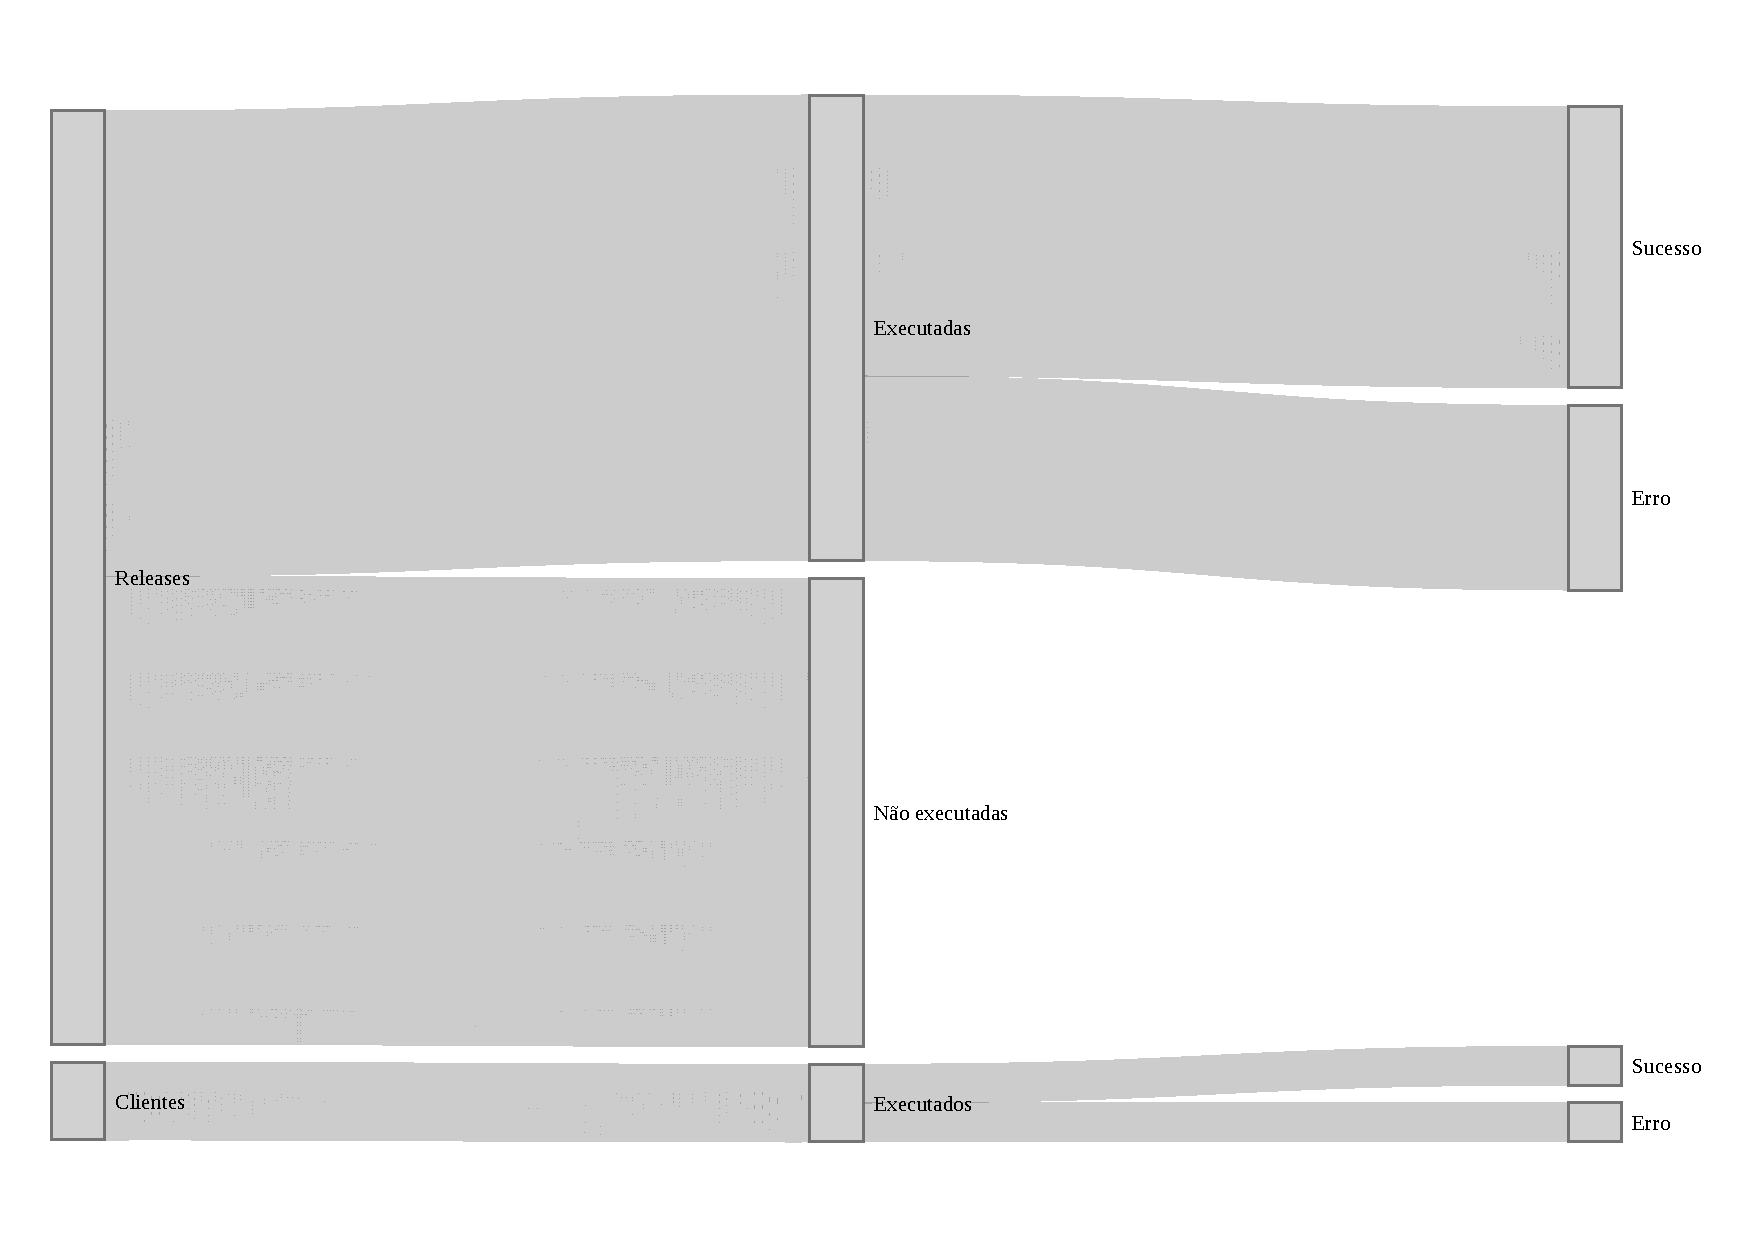
\includegraphics[scale=0.5]{figuras/general_results.pdf}
    \caption{Resultado da execução e da análise manual, por pacotes e por \textit{releases}}
    \label{fig:res_rq1_g}
\end{figure}{}